\chapter{Systemtechnische Lösung}
\label{chapter:Pflichtenheft-SystemtechnischeLoesung}

\section{Lösungsansatz}
\label{section:Pflichtenheft-SystemtechnischeLoesung-Loesungsansatz}

Der erste Schritt ist zu klären, wie die Tabelle im Speicher gespeichert werden soll. Dabei gilt zu beachten, dass unbegrenzt Speicher vorhanden ist und keine Bewertung hinsichtlich des Speichers getroffen wird.

\subsection{Ansatz 1}
Man speichert die Kanalnummer in Register x und die herausgefundene Anzahl Datenbits, die zu dieser Kanalnummer gehören, in Register x+1.

Vorteile:
\begin{itemize}
    \item Man findet sehr schnell zu einer Kanalnummer die entsprechende Anzahl.
    \item Geringer Speicherverbrauch.
\end{itemize}

Nachteile:
\begin{itemize}
    \item Die Kanalnummern werden sehr langsam gefunden, es sei denn man sortiert sie.
    \item Wenn man die Kanalnummern sortiert, muss man die höheren nach hinten verschieben.
\end{itemize}

\subsection{Ansatz 2}
Man speichert in der Speicherzelle mit der Kanalnummer (plus einem Offset, damit das Datenfeld nicht überschrieben wird) als Adresse die herausgefundene Anzahl Datenbits, die zu dieser Kanalnummer gehören.

Vorteile:
\begin{itemize}
    \item Sehr schnelle Bestimmung der Speicheradresse, an der die gewünschte Anzahl steht.
    \item Keine Sortierung notwendig.
    \item Reduzierung des Nettospeicherverbrauchs.
\end{itemize}

Nachteile:
\begin{itemize}
    \item Hoher Bruttospeicherverbrauch, da viele mögliche Nummern unnutzbaren Speicher darstellen.
    \item Schlecht "`per Auge"' ablesbar, weil man die Adresse berechnen muss.
\end{itemize}

Wir haben uns wegen der sehr umständlichen Speicheroperationen gegen den ersten Ansatz entschieden.

Da man nur 32 bits auf einmal auslesen kann, muss man mit der Alu die Operation "`shift"' hinzufügen. Der Offset wird als die Länge des Datenteils festgelegt.

Der Algorithmus ist schematisch in \autoref{figure:Pflichtenheft-SystemtechnischeLoesung-Loesungsansatz-Algorithmus} dargestellt.

\begin{figure}[htb]
    \centering
    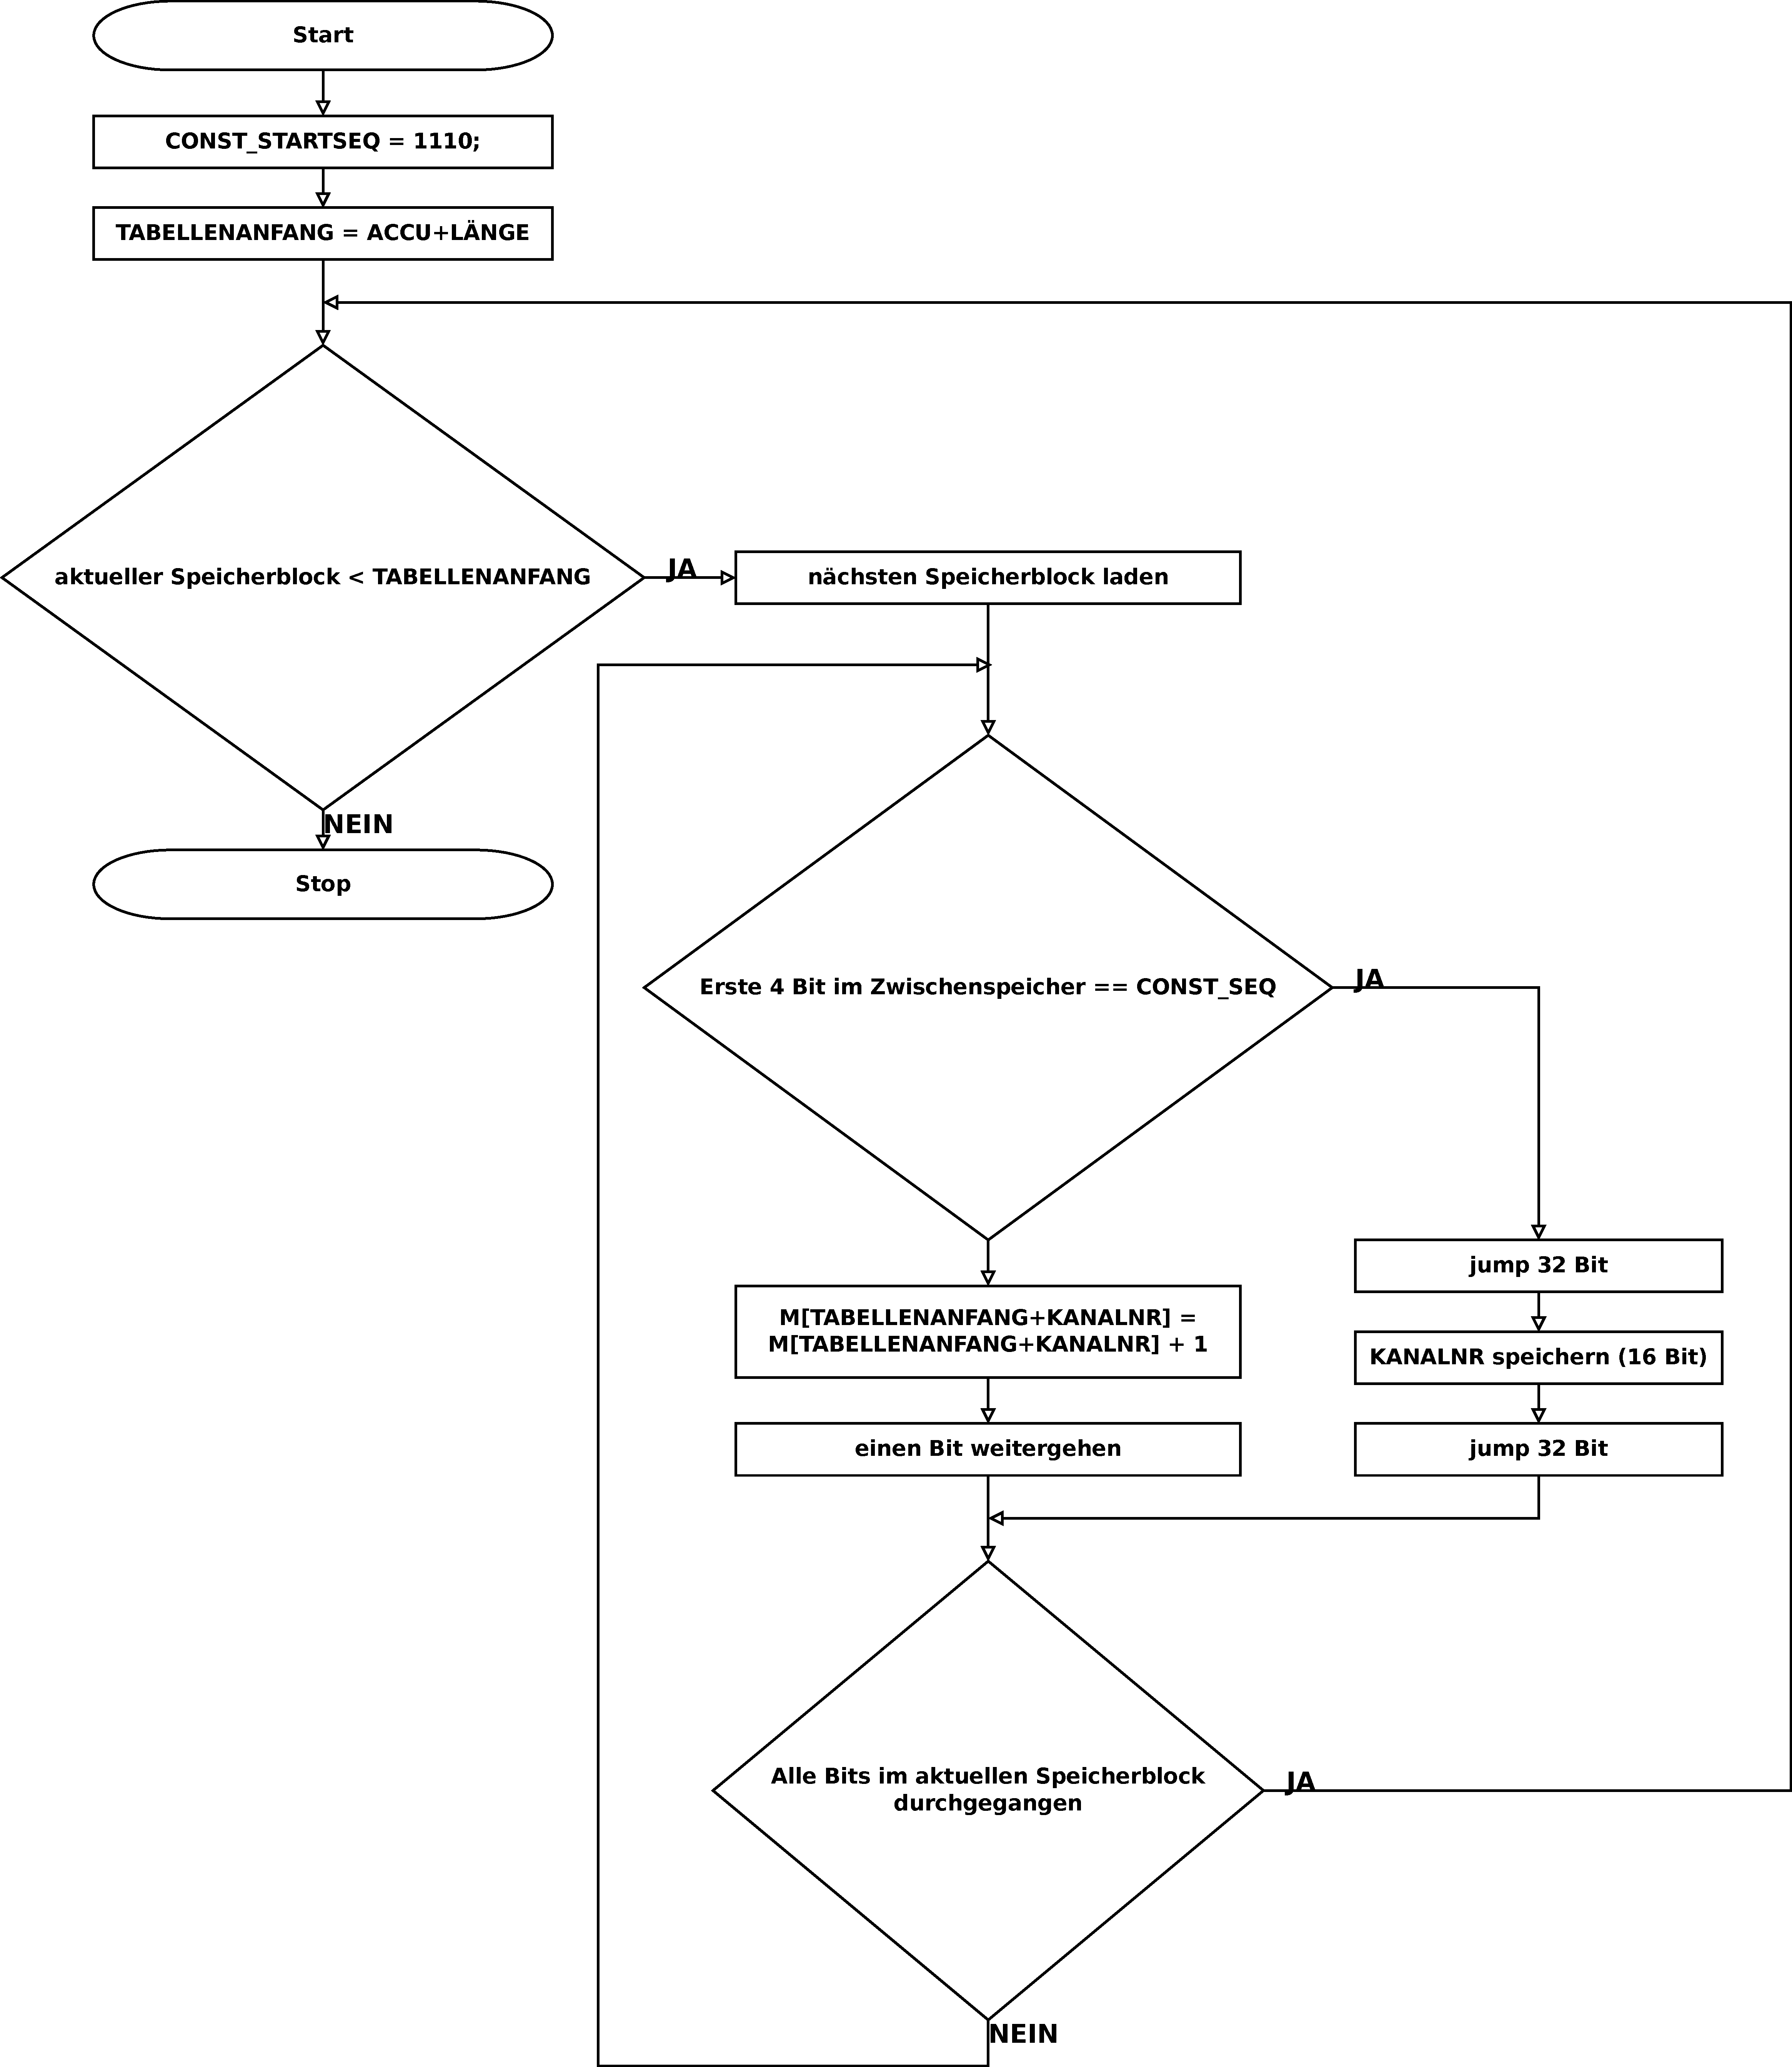
\includegraphics[width=0.7\textwidth, height=0.7\textwidth, draft]{pflichtenheft/res/algorithmus.pdf}
    \caption{Schematischer Aufbau des Algorithmus}
    \label{figure:Pflichtenheft-SystemtechnischeLoesung-Loesungsansatz-Algorithmus}
\end{figure}

\todo{zwei Ansätze, beide kurz erläutern, sich auf einen festlegen (mit Begründung) und ggf. weiter vertiefen.}


\section{Gliederung}
\label{section:Pflichtenheft-SystemtechnischeLoesung-Gliederung}

\todo{Schilderung des Ablaufs der weiteren Entwicklung nach Auftragserteilung. Arbeitszuweisung, Zeitplan, benötigte Ressourcen etc.}


\section[Regulärer Betrieb]{Regulärer Betrieb\footnote{Die folgenden beiden Abschnitte beziehen sich auf den eben gewählten Ansatz}}
\label{section:Pflichtenheft-SystemtechnischeLoesung-regulaer}

Nach Aufruf des Alorithmus mit korrekten Startparametern (siehe \autoref{chapter:Pflichtenheft-Sollzustand}), läuft dieser solange, bis er nach Erreichen der gegebenen Länge des Datenfelds terminiert. Im Hauptspeicher liegt dann eine Tabelle der Kanalnummern und ihrer jeweiligen Datenlänge vor.


\section{Irregulärer Betrieb}
\label{section:Pflichtenheft-SystemtechnischeLoesung-irregulaer}

Eine Reihe von Ereignissen kann zu einem fehlerhaften Verhalten des Algorithmus führen.

\subsection{Fehlerhafte Startparameter}
\label{subsection:Pflichtenheft-SystemtechnischeLoesung-irregulaer-startparameter}

Es kann sein, dass der übergebene Parameter nicht den korrekten Beginn des Datenfeldes beschreibt. In diesem Fall ist nicht vorherzusehen, wie sich der Algorithmus verhält. Man kann allerdings überprüfen, ob der Beginn mit dem Startcode \texttt{1110} beginnt und diesen Fehlerfall somit weitgehend vermeiden.

Falls die angegebene Länge nicht zu den Daten im Hauptspeicher passt, wird entweder ein Teil der Daten vernachlässigt oder undefinierter Speicherinhalt gelesen und dem Ergebnis hinzugefügt. Dies verfälscht zwar das Ergebnis, lässt den Algorithmus jedoch korrekt terminieren. Sofern der Code \texttt{1110} im undefinierten Teil vorkommt, werden u.\,U. weitere falsche Kanäle hinzugefügt oder bereits vorhandene überschrieben (siehe \autoref{subsection:Pflichtenheft-SystemtechnischeLoesung-irregulaer-syntax}).

\subsection{Fehlerhafte Datensyntax}
\label{subsection:Pflichtenheft-SystemtechnischeLoesung-irregulaer-syntax}

Jedes Paket beginnt mit dem Muster \texttt{1110} (vgl. \autoref{chapter:Pflichtenheft-Sollzustand}). Sollte dieses Muster unerwartet \emph{nicht} als Beginn eines Pakets auftreten, arbeitet der Algorithmus vorrübergehend fehlerhaft weiter, bis er wieder auf ein neues Paket mit korrekter Syntax trifft.

Laut Definition der Daten kann \texttt{1110} jedoch nicht an einer solchen falschen Stelle auftreten. Einzige Möglichkeit wäre demzufolge ein fehlerhafter Einsatz des Algorithmus oder eine Beschädigung des Datenfeldes.

\subsection{Modifikation des Datenfeldes während der Laufzeit}
\label{subsection:Pflichtenheft-SystemtechnischeLoesung-irregulaer-moddatenfeld}

Findet während der Laufzeit eine Modifikation des Datenfeldes statt, welches bereits abgearbeitet wurde, so ändert dies das Ergebnis nicht. Eine Modifikation des kommenden Teils führt zu einem verfälschtem Ergebnis (vgl. \autoref{subsection:Pflichtenheft-SystemtechnischeLoesung-irregulaer-startparameter}).

\subsection{Modifikation des Tabellenteils während der Laufzeit}
\label{subsection:Pflichtenheft-SystemtechnischeLoesung-irregulaer-modtabelle}

Eine Modifikation der Ergebnistabelle während der Laufzeit führt zu fehlerhaften Datenlängen in der Tabelle.
